\documentclass[11pt,letterpaper]{article}
\usepackage[utf8]{inputenc}
\usepackage{amsmath,amssymb,fullpage,graphicx}

\let\hat\widehat
\let\tilde\widetilde
\begin{document}
\subsection*{Lect 6-1}
\begin{verbatim}
type_one <- c(65, 81, 57, 66, 82, 82, 67, 59, 75, 70)
type_two <- c(64, 71, 83, 59, 65, 56, 69, 74, 82, 79)
n1 <- length(type_one)
n2 <- length(type_two)
s1 <- sd(type_one)
s2 <- sd(type_two)
\end{verbatim}
\subsection*{a}
\noindent $H_0: \mu_1 = \mu_2$ \\
\noindent $H_1: \mu_1 \neq \mu_2$, a two-tails t-test \\

\noindent With the assumption of equal variance, we can calculate the pooled sample variance. 
\begin{align*}
s_p^2 &= \frac{(n_1 - 1)s_1^2 + (n_2 - 1)s_2^2}{(n_1 - 1) +  (n_2 - 1)} \\
t &= \frac{(\bar{Y_1} - \bar{Y_2}) - (\mu_1 - \mu_2)}{s_p \sqrt{1/n_1 + 1/n_2}} \\
t & \sim t_{(n_1 + n_2 - 2)}
\end{align*}
\noindent Sample standard error $se = s_p\sqrt{\frac{1}{n_1} + \frac{1}{n_2}}$  
\begin{verbatim}
sp <- sqrt(((n1-1)*s1^2 + (n2-1)*s2^2)/(n1 + n2 - 2))
se <- sp * sqrt(1/n1 + 1/n2)
t_obs <- (mean(type_one) - mean(type_two)) / se

> mean(type_one) - mean(type_two)
[1] 0.2
> sp
[1] 9.315459
> se
[1] 4.166
> t_obs
[1] 0.04800768
\end{verbatim}

\noindent Plug in the data, we get $(\bar{Y_1} - \bar{Y_2}) = 0.2$, $s_p = 9.315459$, standard error $= 4.166$, observed t-statistic $= 0.04800768$

\begin{verbatim}
alpha <- 0.05
low_cv <- qt(alpha/2, df = (n1 + n2 - 2)) 
up_cv <- qt(1 - alpha/2, df = (n1 + n2 - 2))

> low_cv
[1] -2.100922
> up_cv
[1] 2.100922
\end{verbatim}

\noindent The lower critical value for t-statistic is $-2.100922$ and the upper critical value is $2.100922$. Under the significant level of 0.05, rejection regions are $t_{obs} < -2.100922$ or $t_{obs} > 2.100922$. Because $t_{obs} = 0.048$ does not fall in any of the above regions, therefore, this sample data cannot be significant evidence against $H_0$.

\begin{verbatim}
CI_low <- (mean(type_one) - mean(type_two)) - qt(1 - alpha/2, df = (n1 + n2 - 2)) * se
CI_up <- (mean(type_one) - mean(type_two)) + qt(1 - alpha/2, df = (n1 + n2 - 2)) * se
> CI_low
[1] -8.552441
> CI_up
[1] 8.952441
\end{verbatim}

\noindent We are $95 \%$ confident that true difference in population means fall in the region $[-8.552441, 8.952441]$. Since $H_0: \mu_1 - \mu_2 = 0$ is within this confidence interval, the sample data does not provide significant evidence to reject $H_0$.

\begin{verbatim}
p_val <- (1 - pt(t_obs, df=n1+n2-2)) * 2
> p_val
[1] 0.9622388
\end{verbatim}

\noindent Observed t-statistic has a p-value of $0.9622388$, which is larger than significant level $\alpha = 0.05$. Therefore, sample data fail to provide significant evidence to reject $H_0$

\subsection*{b}
\noindent $H_0: \sigma_1 = \sigma_2$ \\
\noindent $H_1: \sigma_1 \neq \sigma_2$ \\

\noindent A two variance two-tail F-test can be applied here. $F = s_1^2 /s_2^2$ with $df1= 9, df2= 9$
\begin{verbatim}
F_obs <- s1^2 / s2^2
p_val <- pf(F_obs, df1=n1-1, df2=n2-1) +
  (1 - pf(1 + abs(F_obs - 1), df1=n1-1, df2=n2-1))

> F_obs
[1] 0.9782168
> p_val
[1] 0.9746426
\end{verbatim}
The sample F-statistic has a value of $0.9782168$, having a p-value of $0.9746$. Under significance level of $0.05$, the data fail to provide strong evidence against $H_0$, since p-value $> \alpha$.  \\

The $\alpha$ level confidence interval of F-statistic is 
\begin{align*}
P (F_{\frac{\alpha}{2}} < F_{obs} < F_{1 - \frac{\alpha}{2}}) &= 1 - \alpha \\
P (F_{\frac{\alpha}{2}} < \frac{s_1^2 / \sigma_1^2}{s_2^2 / \sigma_2^2} < F_{1 - \frac{\alpha}{2}}) &= 1 - \alpha \\
P (\frac{s_2^2}{s_1^2} F_{\frac{\alpha}{2}} < \frac{\sigma_2^2}{\sigma_1^2} < \frac{s_2^2}{s_1^2} F_{1-\frac{\alpha}{2}} ) &= 1 - \alpha \\
P (\frac{s_1^2}{s_2^2} \frac{1}{F_{1 - \frac{\alpha}{2}}} < \frac{\sigma_1^2}{\sigma_2^2} < \frac{s_1^2}{s_2^2} \frac{1}{F_{ \frac{\alpha}{2}}} ) &= 1 - \alpha
\end{align*}
\noindent The lower confidence limit is $\frac{s_1^2}{s_2^2} \frac{1}{F_{1 - \frac{\alpha}{2}}}$, the upper confidence limit is $\frac{s_1^2}{s_2^2} \frac{1}{F_{ \frac{\alpha}{2}}}$
\begin{verbatim}
CI_low <- s1^2 / s2^2 * 1 / qf(1 - alpha/2, df1=n1-1, df2=n2-1)
CI_up <- s1^2 / s2^2 * 1 / qf(alpha/2, df1=n1-1, df2=n2-1)

> CI_low
[1] 0.2429752
> CI_up
[1] 3.938295
\end{verbatim}
\noindent We are $95 \%$ confident that $\sigma_1^2 / sigma_2^2$ is in $[0.2429752, 3.938295]$. 

\noindent Since $H_0: \frac{\sigma_1^2}{\sigma_2^2} = 1$ falls in the $95 \%$ confidence interval, the observed statistic fail to provide strong evidence against the null. 

\begin{verbatim}
low_cv <- qf(alpha/2, df1=n1-1, df2=n2-1)
up_cv <- qf(1 - alpha/2, df1=n1-1, df2=n2-1)
> low_cv
[1] 0.2483859
> up_cv
[1] 4.025994
\end{verbatim}
\noindent The rejection region under significance level $95 \%$ is $s_1^2 / s_2^2 < 0.2483859$ or $s1^2 / s_2^2 >4.025994 $. Since observed F-statistic $0.978$ does not fall in any of the rejection regions, we may conclude that the sample data fail to show significant evidence against $H_0$.


\subsection*{Lect 6-2}
\begin{align*}
SS_{Treat} &= n \sum_{i}^a (\bar{Y_{i.}} - \bar{Y_{..}})^2 \\
&= n \sum_{i}^a (\bar{Y_{i.}}^2 + \bar{Y_{..}}^2 - 2 \bar{Y_{i.}} \bar{Y_{..}}) \\
&=  n \sum_{i}^a \bar{Y_{i.}}^2 + n \sum_{i}^a \bar{Y_{..}}^2 - 2 n \sum_{i}^a\bar{Y_{i.}} \bar{Y_{..}} 
\end{align*}

\noindent Note that $\bar{Y_{i.}} = \frac{1}{n} \sum_j^n Y_{ij}$, and $Y_{i.} = \sum_j^n Y_{ij}$ 

\begin{align*}
n \sum_{i}^a \bar{Y_{i.}}^2 &= n \sum_{i}^a (\frac{1}{n} \sum_j^n Y_{ij})^2 \\
&= n (\frac{1}{n})^2 \sum_{i}^a (\sum_j^n Y_{ij})^2 \\
&= \frac{1}{n} \sum_{i}^a Y_{i.}^2
\end{align*}

\noindent Note that $\bar{Y_{..}} = \frac{1}{na} \sum_i^a \sum_j^n Y_{ij}$, and $Y_{..} = \sum_i^a \sum_j^n Y_{ij}$ 

\begin{align*}
n \sum_{i}^a \bar{Y_{..}}^2 &= n \bar{Y_{..}}^2 \sum_i^a 1 \\
&= na \bar{Y_{..}}^2 \\
&= na  (\frac{1}{na} \sum_i^a \sum_j^n Y_{ij})^2 \\
&= \frac{1}{na} Y_{..}^2
\end{align*}
\begin{align*}
2 n \sum_{i}^a\bar{Y_{i.}} \bar{Y_{..}}  &= 2 n \sum_i^a (\frac{1}{n} \sum_j^n X_{ij}) (\frac{1}{na} \sum_i^a \sum_j^n Y_{ij}) \\
&= 2n \cdot \frac{1}{n} \cdot \frac{1}{na} (\sum_i^a \sum_j^n X_{ij}) ( \sum_i^a \sum_j^n Y_{ij}) \\
&= \frac{2}{na} Y_{..}^2
\end{align*}
\begin{align*}
SS_{Treat} &= n \sum_{i}^a \bar{Y_{i.}}^2 + n \sum_{i}^a \bar{Y_{..}}^2 - 2 n \sum_{i}^a\bar{Y_{i.}} \bar{Y_{..}}  \\
&=  \frac{1}{n} \sum_{i}^a Y_{i.}^2 + \frac{1}{na} Y_{..}^2 - \frac{2}{na} \bar{Y_{..}}^2 \\
&= \frac{1}{n} \sum_{i}^a Y_{i.}^2 - \frac{1}{N}Y_{..}^2
\end{align*}

\subsection*{Lect 6-3}
\begin{align*}
F &= \frac{an}{a-1} \frac{\sum_i^a (\bar{Y_{i.}} - \bar{Y_{..}})^2}{\sum_i^a s_i^2} \\
\text{when (a = 2) } F &= 2n \frac{ (\bar{Y_{1.}} - \bar{Y_{..}})^2 + (\bar{Y_{2.}} - \bar{Y_{..}})^2}{s_1^2 + s_2^2} \\
&= 2n \frac{\bar{Y_{1.}}^2 + \bar{Y_{..}}^2 - 2 \bar{Y_{1.}}\bar{Y_{..}} + \bar{Y_{2.}}^2 + \bar{Y_{..}}^2 - 2 \bar{Y_{2.}}\bar{Y_{..}}     }{s_1^2 + s_2^2} \\
&= 2n \frac{\bar{Y_{1.}}^2 + \bar{Y_{2.}}^2 + 2 \bar{Y_{..}}^2 - 2 \bar{Y_{1.}}\bar{Y_{..}} - 2 \bar{Y_{2.}}\bar{Y_{..}}}{s_1^2 + s_2^2} \\
\end{align*}
Note that $\bar{Y_{..}} = \frac{1}{2} (\bar{Y_{1.}} + \bar{Y_{2.}})$, substitute this value into the equation.
\begin{align*}
2 \bar{Y_{..}}^2 &= 2 (\frac{1}{2} (\bar{Y_{1.}} + \bar{Y_{2.}}))^2 \\
&= \frac{1}{2} (\bar{Y_{1.}} + \bar{Y_{2.}})^2 \\
&= \frac{1}{2} (\bar{Y_{1.}}^2 + \bar{Y_{2.}}^2 + 2 \bar{Y_{1.}}\bar{Y_{2.}}) \\
&= \frac{1}{2} \bar{Y_{1.}}^2 + \frac{1}{2} \bar{Y_{2.}}^2 + \bar{Y_{1.}}\bar{Y_{2.}} 
\end{align*}
\begin{align*}
-2 \bar{Y_{1.}}\bar{Y_{..}} &= -2 \bar{Y_{1.}} (\frac{1}{2} (\bar{Y_{1.}} + \bar{Y_{2.}})) \\
&= - \bar{Y_{1.}} ^2 - \bar{Y_{1.}} \bar{Y_{2.}} 
\end{align*}
\begin{align*}
-2 \bar{Y_{2.}}\bar{Y_{..}} &= -2 \bar{Y_{2.}} (\frac{1}{2} (\bar{Y_{1.}} + \bar{Y_{2.}})) \\
&= - \bar{Y_{2.}} ^2 - \bar{Y_{1.}} \bar{Y_{2.}} 
\end{align*}
\begin{align*}
F &= 2n \frac{\bar{Y_{1.}}^2 + \bar{Y_{2.}}^2 + \frac{1}{2} \bar{Y_{1.}}^2 + \frac{1}{2} \bar{Y_{2.}}^2 + \bar{Y_{1.}}\bar{Y_{2.}} - \bar{Y_{1.}} ^2 - \bar{Y_{1.}} \bar{Y_{2.}}  - \bar{Y_{2.}} ^2 - \bar{Y_{1.}} \bar{Y_{2.}} }{s_1^2 + s_2^2} \\
&= 2n \frac{\frac{1}{2} \bar{Y_{1.}}^2 + \frac{1}{2	} \bar{Y_{2.}}^2 -  \bar{Y_{1.}} \bar{Y_{2.}} }{s_1^2 + s_2^2} \\
&= n \frac{\bar{Y_{1.}}^2 + \bar{Y_{2.}}^2 -  2\bar{Y_{1.}} \bar{Y_{2.}} }{s_1^2 + s_2^2} \\
&= \frac{(\bar{Y_{1.}} - \bar{Y_{2.}})^2}{(s_1^2 + s_2^2) / n}
\end{align*}
Note that $s_p^2 = \frac{1}{2}(s_1^2 + s_2^2)$, substitute $2 \cdot s_p^2$ for $(s_1^2 + s_2^2)$
\begin{align*}
F &=  \frac{(\bar{Y_{1.}} - \bar{Y_{2.}})^2}{s_p^2 \cdot  2/n} = t^2 \text{, when a = 2}
\end{align*}

\subsection*{Lect 6-4}
\begin{align*}
E(\bar{Y^2}) - E(\bar{Y}^2) &= E(\frac{1}{n} \sum_i^n Y_i^2) - E((\frac{1}{n} \sum_i^n Y_i)^2) \\
&= \frac{1}{n} E(\sum_i^n Y_i^2) - \frac{1}{n^2} E((\sum_i^n Y_i) ^2) \\
&= \frac{1}{n}\sum_i^n E( Y_i^2) - \frac{1}{n^2} E((\sum_i^n Y_i) (\sum_i^n Y_i)) \\
\end{align*}
\noindent Note that $Y_i's$ are identical, therefore, $E(Y_i^2) = E(Y^2)$
\begin{align*}
\frac{1}{n}\sum_i^n E( Y_i^2) &= \frac{1}{n} E(Y^2) \sum_i^n 1 \\
&= E(Y^2) \\
\frac{1}{n^2} E((\sum_i^n Y_i) (\sum_i^n Y_i)) &= \frac{1}{n^2} E(\sum_i^n Y_i^2 + 2 \cdot \sum_{j>i}^n Y_iY_j) \\
&= \frac{1}{n^2} E( \sum_i^n Y_i^2 ) + \frac{2}{n^2} E(\sum_{j>i}^n Y_iY_j) \\
&= \frac{1}{n^2}\sum_i^n  E( Y_i^2 ) + \frac{2}{n^2} \sum_{j>i}^n E(Y_iY_j) 
\end{align*}
Note that $Y_i's$ are independent, $E(Y_iY_j) = E(Y_i)E(Y_j)$. $Y_i's$ are identical, therefore, $E(Y_i) = E(Y_j)=E(Y)$.
\begin{align*}
\frac{1}{n^2} E((\sum_i^n Y_i) (\sum_i^n Y_i)) &= \frac{2}{n^2} E(Y_i) E(Y_j) \sum_i^n 1 + \frac{1}{n^2} E(Y)^2 \sum_{j>i}^n 1 \\
&= \frac{1}{n} E(Y^2) + \frac{2}{n^2} \frac{n(n-1)}{2} E(Y)^2 \\
&= \frac{1}{n} E(Y^2) + \frac{n-1}{n} E(Y)^2 
\end{align*} 
\begin{align*}
E(\bar{Y^2}) - E(\bar{Y}^2) &= \frac{1}{n}\sum_i^n E( Y_i^2) - \frac{1}{n^2} E((\sum_i^n Y_i) (\sum_i^n Y_i)) \\
&= E(Y^2 -  \frac{1}{n} E(Y^2) - \frac{n-1}{n} E(Y)^2 \\
&= \frac{n-1}{n} (E(Y^2) - E(Y)^2) \\
&= \frac{n-1}{n} Var(Y)
\end{align*} 

\subsection*{Lect 7-1}
\subsection*{a}
\begin{verbatim}
tr_level <- as.factor(rep(c(1,2,3,4), each=10))
pool_dt <- data.frame(tr_level, as.vector(t(y)))
plot(pool_dt, xlab='Treatment Levels', ylab='Y values')
\end{verbatim}
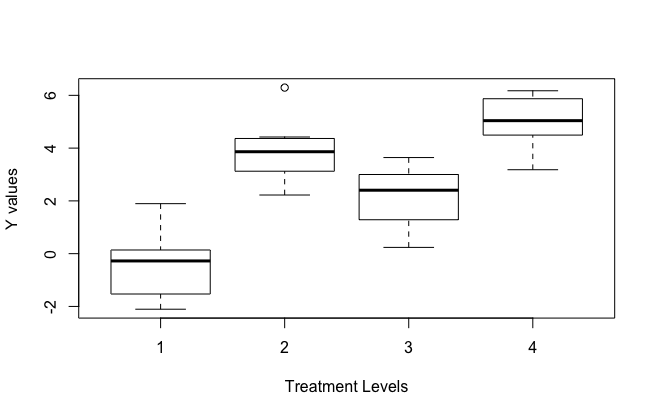
\includegraphics[scale=0.45]{lect-7-1-a.png}

\noindent If the hypothesis looks like $H_0: \mu_1 = \mu_2 = \mu_3 = \mu_4$, $H_1:$ there are at least two means are different, then base on this boxplot, $X$ do have effect on $Y$, since the range of 1 doesn't have any overlap with box of 4, indicating that the true mean $\mu_1$ are unlikely equal to $\mu_4$  \\

\subsection*{b}
\begin{verbatim}
grand_mean <- mean(pool_dt[,2])
new_dt <- data.frame(tr_level, pool_dt[,2] - grand_mean)
plot(new_dt, xlab='Treatment Levels', ylab='Yij - Grand Mean')
\end{verbatim}
\includegraphics[scale=0.45]{lect-7-1-b.png}

\noindent  The distribution of data on boxplot resembles boxplot in part a, the range of $y_1$ does not overlap range of $y_4$, indicating that the true mean $\mu_1$ are unlikely equal to $\mu_4$. Therefore, the sample data provide significant evidence against the equal means hypothesis, showing that $X$ has effect on $Y$.\\

\subsection*{c}
\begin{verbatim}
y_bar <- apply(y, 1, mean)
y_effect <- y_bar - grand_mean

> y_bar
[1] -0.3537095  3.9038404  2.1095378  5.0102435
> y_effect
[1] -3.0211875  1.2363624 -0.5579403  2.3427655
\end{verbatim}

\subsection*{d}
\begin{verbatim}
y_sd <- apply(y, 1, sd)
y_se <- y_sd / sqrt(10)

> y_se
[1] 0.3933592 0.3433781 0.3964595 0.2976147
\end{verbatim}

\subsection*{e}
\begin{verbatim}
one_sd_bd <- c(y_effect + y_se, y_effect - y_se)
tr_level <- as.factor(rep(c(1,2,3,4), 2))
effect_est <- data.frame(tr_level, one_sd_bd)
plot(effect_est, xlab='Treatment Levels', ylab='Effects')
abline(h=0, lty=2)
\end{verbatim}
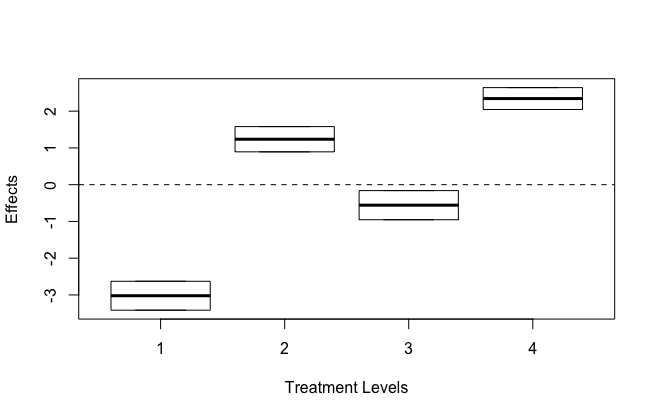
\includegraphics[scale=0.5]{lect-7-1-e.png}

\noindent From the plot we can perceive that none of the intervals $\bar{\tau_i} \pm se$ covers 0. In this case, it looks like none of the effect can be zero, i.e. zero is in none of the confidence intervals, providing evidence that $X$ has effect on $Y$.

\subsection*{f}
\begin{align*}
SS_{treat} &= n \sum_i^a (\bar{Y_{i.}} - \bar{Y_{..}}) \\
SS_e &= (n-1) \sum_i^a s_i^2
\end{align*}
\begin{verbatim}
SStr <- 10 * sum((y_bar - grand_mean)^2)
SSe <- (10 - 1) * sum(y_sd^2)
> SStr
[1] 164.5601
> SSe
[1] 46.65552
\end{verbatim}
\begin{align*}
F_{obs} &= \frac{MS_{tr}}{MS_e} = \frac{SS_{tr} / (a - 1)}{SS_e / (N - a)} 
\end{align*}
\begin{verbatim}
F_obs <- (SStr / (4-1)) / (SSe / (40 - 4))
> F_obs
[1] 42.32557
\end{verbatim}
\noindent The F-statistic is 42.33. 
\begin{verbatim}
> qf(0.95, df1=3, df2=36, lower.tail = T)
[1] 2.866266
\end{verbatim}
\noindent The critical value is 2.866266, which implies if $\tau_1 = \tau_2 = \tau_3 = \tau_4 = 0$, then the probability of getting more extreme F-statistic than 2.866266 is only $0.05$. Since observed F-statistic is 42.33, falling in rejection region, it is a strong evidence that at least one of the effects is non-zero.

\subsection*{Lect 7-2}
\subsection*{a}
\begin{align*}
E(\hat{\tau_i}) &= E(\bar{Y_{i.}} - \bar{Y_{..}}) \\
&= E( \frac{1}{n} \sum_j^n Y_{ij}  - \frac{1}{na} \sum_{j}^n \sum_k^a Y_{kj}) \\
&= \frac{1}{n} \sum_j^n E( Y_{ij})  - \frac{1}{na} \sum_{j}^n \sum_k^a E( Y_{kj}) \\
&= \frac{1}{n} \sum_j^n E(\mu + \tau_i + \epsilon_{ij}) - \frac{1}{na} \sum_{j}^n \sum_k^a E( Y_{kj}) \\
\end{align*}
\noindent Note that in this model $E(\epsilon_{ij}) = 0$, $\mu$ and $\tau_i$ are parameters, $E(Y_{kj}) = \mu$ for $k = 1, 2, ... a$, $Y_{kj}$ is pooled data. 
\begin{align*}
E(\hat{\tau_i}) &=  \frac{1}{n} (\sum_j^n 1) (\mu + \tau_i + 0) - \frac{1}{na} (\sum_{j}^n \sum_k^a 1) \mu \\
&= \tau_i
\end{align*}
\begin{align*}
Var(\hat{\tau_i}) &= V(\bar{Y_{i.}} - \bar{Y_{..}}  ) \\
&= V(\frac{1}{n} \sum_j^n Y_{ij} - \frac{1}{na} \sum_k^a \sum_j^n Y_{kj}) \\
&= V(\frac{1}{n} \sum_j^n (\mu + \tau_i + \epsilon_{ij})- \frac{1}{na} \sum_k^a \sum_j^n (\mu + \tau_k + \epsilon_{kj})) \\
&= V(\mu + \tau_i + \sum_j^n \epsilon_{ij} - \mu - \bar{\tau_k} - \sum_k^a \sum_j^n \epsilon_{kj} ) \\
\end{align*}
\noindent Note that $\mu$, $\tau_i$, $\bar{\tau_i}$ are parameters, and $Var(x + c) = Var(x)$ for any constant c.
\begin{align*}
Var(\hat{\tau_i}) &= Var( \bar{\epsilon_{i.}} - \bar{\epsilon_{..}} ) = \frac{a-1}{an} \sigma_{\epsilon}^2
\end{align*}

\subsection*{b}
With assumption that $\hat{\tau_i}$ is normal, $\sigma_{\epsilon}$ is known.

\noindent Then $Z = \frac{(\hat{\tau_i}) - (\tau_i)  }{\sqrt{\frac{a-1}{an} \cdot \sigma_{\epsilon}^2} } \sim N(0, 1)$, $\bar{Y_{i.}} - \bar{Y_{..}}$ is an unbiased estimator for $\tau_i$.
\begin{align*}
& P(Z_{\frac{\alpha}{2}} < Z_{obs} < Z_{\frac{\alpha}{2}}) = 1 - \alpha \\
& P(Z_{\frac{\alpha}{2}} <  \frac{(\bar{Y_{i.}} - \bar{Y_{..}}) - (\tau_i)  }{\sqrt{\frac{a-1}{an} \cdot \sigma_{\epsilon}^2} } < Z_{\frac{\alpha}{2}}) = 1 - \alpha \\
& P( Z_{\frac{\alpha}{2}} \sqrt{\frac{a-1}{an} \cdot \sigma_{\epsilon}^2} < \bar{Y_{i.}} - \bar{Y_{..}} - \tau_i < Z_{1-\frac{\alpha}{2}} \sqrt{\frac{a-1}{an} \cdot \sigma_{\epsilon}^2}) = 1 - \alpha \\
& P( Z_{\frac{\alpha}{2}} \sqrt{\frac{a-1}{an} \cdot \sigma_{\epsilon}^2} - ( \bar{Y_{i.}} - \bar{Y_{..}})<  - \tau_i < Z_{1-\frac{\alpha}{2}} \sqrt{\frac{a-1}{an} \cdot \sigma_{\epsilon}^2} - ( \bar{Y_{i.}} - \bar{Y_{..}})) = 1 - \alpha \\
& P( ( \bar{Y_{i.}} - \bar{Y_{..}}) - Z_{\frac{\alpha}{2}} \sqrt{\frac{a-1}{an} \cdot \sigma_{\epsilon}^2} > \tau_i > ( \bar{Y_{i.}} - \bar{Y_{..}}) - Z_{1-\frac{\alpha}{2}} \sqrt{\frac{a-1}{an} \cdot \sigma_{\epsilon}^2} ) = 1 - \alpha \\
& P( ( \bar{Y_{i.}} - \bar{Y_{..}}) + Z_{\frac{\alpha}{2}} \sqrt{\frac{a-1}{an} \cdot \sigma_{\epsilon}^2} < \tau_i < ( \bar{Y_{i.}} - \bar{Y_{..}}) - Z_{\frac{\alpha}{2}} \sqrt{\frac{a-1}{an} \cdot \sigma_{\epsilon}^2} ) = 1 - \alpha \\
\end{align*}
\noindent We are $(1-\alpha) \%$ confident that the effect $\tau_i$ at $X = i$ is in the interval \\ 
$[ ( \bar{Y_{i.}} - \bar{Y_{..}}) + Z_{\frac{\alpha}{2}} \sqrt{\frac{a-1}{an} \cdot \sigma_{\epsilon}^2} , ( \bar{Y_{i.}} - \bar{Y_{..}}) - Z_{\frac{\alpha}{2}} \sqrt{\frac{a-1}{an} \cdot \sigma_{\epsilon}^2} ]$

\subsection*{c}
\begin{align*}
Var(\bar{\epsilon_{i.}}  - \bar{\epsilon_{..}}) &= V(\frac{1}{n} \sum_j^n \epsilon_{ij} - \frac{1}{na} \sum_k^a \sum_j^n \epsilon_{kj}) \\
&= V(\frac{1}{n} \sum_j^n \epsilon_{ij} - \frac{1}{na} (\sum_{k \neq i}^a \sum_j^n \epsilon_{kj} + \sum_j^n \epsilon_{ij})) \\
&= V(\sum_j^n \epsilon_{ij} (\frac{1}{n} - \frac{1}{na}) - \frac{1}{na} \sum_{k \neq i} \sum_j^n \epsilon_{kj}  ) \\
&= V(\sum_j^n \epsilon_{ij} (\frac{1}{n} - \frac{1}{na})) + V(\frac{1}{na} \sum_{k \neq i}^a \sum_j^n \epsilon_{kj} ) - 2 Cov(\sum_j^n \epsilon_{ij} (\frac{1}{n} + \frac{1}{na}), \frac{1}{na} \sum_{k \neq i} \sum_j^n \epsilon_{kj})
\end{align*}
\noindent Since $\epsilon$ is independent, and $\sum_j^n \epsilon_{ij}$ are disjoint with $\sum_{k \neq i}^a \sum_j^n \epsilon_{kj}$, $Cov(\sum_j^n \epsilon_{ij} (\frac{1}{n} + \frac{1}{na}), \frac{1}{na} \sum_{k \neq i} \sum_j^n \epsilon_{kj})$ is equal to zero.

\begin{align*}
Var(\bar{\epsilon_{i.}}  - \bar{\epsilon_{..}}) &= V(\sum_j^n \epsilon_{ij} (\frac{1}{n} - \frac{1}{na})) + V(\frac{1}{na} \sum_{k \neq i}^a \sum_j^n \epsilon_{kj} ) \\
&= (\frac{a-1}{na})^2 \sum_j^n V(\epsilon_{ij}) + \frac{1}{(na)^2} \sum_{k \neq i}^a \sum_j^n V( \epsilon_{kj} ) \\
\end{align*}
\noindent Note that $\epsilon$ is iid and follows normal distribution with variance of $\sigma_{\epsilon}$. $Var(\epsilon_{ij}) = Var(\epsilon_{kj}) = Var(\epsilon) = \sigma^2_{\epsilon}$
\begin{align*}
Var(\bar{\epsilon_{i.}}  - \bar{\epsilon_{..}}) &= \frac{(a-1)^2}{n^2 a^2} \sigma^2 \sum_j^n 1 + \frac{1}{n^2 a^2} \sigma \sum_{k \neq i}^2 \sum_j^n 1 \\
&= ( \frac{(a-1)^2}{na^2} + \frac{(a-1)}{na^2} ) \sigma^2 \\
&= \frac{a-1}{na} \sigma^2
 \end{align*}

\subsection*{Lect 7-3}
\subsection*{a}
\begin{align*}
E(MS_{Tr}) &= E(\frac{n}{a-1} \sum_i^a (\bar{Y_{i.}} - \bar{Y_{..}})^2 ) \\
&= \frac{n}{a-1} E(\sum_i^a (\frac{1}{n} \sum_j^n Y_{ij}  - \frac{1}{na} \sum_i^a \sum_j^n Y_{ij} )^2 ) \\
&= \frac{n}{a-1} E(\sum_i^a (\frac{1}{n} \sum_j^n (\mu + \tau_i +  \epsilon_{ij}) -  \frac{1}{na} \sum_i^a \sum_j^n \mu + \tau_i + \epsilon_{ij} )^2 ) \\
&= \frac{n}{a-1} E[ \sum_i^a (\mu + \tau_i + (\frac{1}{n} \sum_j^n  \epsilon_{ij}) - \mu - \frac{1}{n} \sum_j^n ( \frac{1}{a}\sum_i^a \tau_i + \frac{1}{a} \sum_i^a  \epsilon_{ij} ) )^2 ] \\
&= \frac{n}{a-1} E[ \sum_i^a (\mu + \tau_i + \bar{\epsilon_{i.}} - \mu - \bar{\tau_i} - \frac{1}{an} \sum_j^n \sum_i^a  \epsilon_{ij} )^2 ] \\
&= \frac{n}{a-1} E[ \sum_i^a (\mu + \tau_i + \bar{\epsilon_{i.}} - \mu - \bar{\tau_.} - \bar{\epsilon_{..}} )^2 ] \\
&= \frac{n}{a-1} E[ \sum_i^a ( \tau_i + \bar{\epsilon_{i.}} - \bar{\tau_.} - \bar{\epsilon_{..}} )^2 ] 
\end{align*}

\subsection*{b}
\begin{align*}
E(\sum_i^a (\bar{\epsilon_{i.}} - \bar{\epsilon_{..}})^2 ) &= \sum_i^aE( (\bar{\epsilon_{i.}} - \bar{\epsilon_{..}})^2 ) \\
&= \sum_i^a (Var( \bar{\epsilon_{i.}} - \bar{\epsilon_{..}})  + E(\bar{\epsilon_{i.}} - \bar{\epsilon_{..}})^2) 
\end{align*}
\noindent We have proved $Var(\bar{\epsilon_{i.}} - \bar{\epsilon_{..}}) = \frac{a-1}{na} \sigma_{\epsilon}^2$. \\

\noindent $E(\bar{\epsilon_{i.}} - \bar{\epsilon_{..}} ) = E(\bar{\epsilon_{i.}}) - E( \bar{\epsilon_{..}}) = \frac{1}{n} \sum_j^n E(\epsilon_{ij})$, since $\epsilon$ is iid, $E(\epsilon_{ij}) = E(\epsilon) = 0$, $E(\bar{\epsilon_{i.}} - \bar{\epsilon_{..}}) = 0$
\begin{align*}
E(\sum_i^a (\bar{\epsilon_{i.}} - \bar{\epsilon_{..}})^2 ) &= \sum_i^a \frac{a-1}{na} \sigma_{\epsilon}^2 = \frac{a-1}{n} \sigma_{\epsilon}^2
\end{align*}

\subsection*{c}
\begin{align*}
E(\sum_i^a (\tau_i - \bar{\tau_.} )^2) &= \sum_i^a E(\tau_i - \bar{\tau_.} )^2) \\
&= \sum_i^a (Var(\tau_i - \bar{\tau_.}) + E(\tau_i - \bar{\tau_.} )^2)
\end{align*}
\noindent Note that $\tau_i$'s are parameters, $\bar{tau_.}$ is constant, therefore, $Var(\tau_i - \bar{\tau_.}) = 0$. $E(\tau_i) = \tau_i$, $ E( \bar{\tau_.}) = \bar{\tau_.}$
\begin{align*}
E(\sum_i^a (\tau_i - \bar{\tau_.} )^2) &= \sum_i^a (0 + (\tau_i - \bar{\tau_.})^2 ) = \sum_i^a (\tau_i - \bar{\tau_.})^2
\end{align*}

\subsection*{d}
\begin{align*}
2E[\sum_i^a (\tau_i - \bar{\tau_.}) (\bar{\epsilon_{i.}} - \bar{\epsilon_{..}} ) ] &= 2 \sum_i^a E [(\tau_i - \bar{\tau_.}) (\bar{\epsilon_{i.}} - \bar{\epsilon_{..}} )] \\
&= 2 \sum_i^a (\tau_i - \bar{\tau_.}) E( \bar{\epsilon_{i.}} - \bar{\epsilon_{..}} ) \\
\end{align*}
\noindent $\tau_i$ and $\bar{\tau_.}$ are constant numbers, therefore, $E(\tau_i - \bar{\tau_.}) = \tau_i - \bar{\tau_.}$. We have proved that $E(\bar{\epsilon_{i.}} - \bar{\epsilon_{..}}) = 0$
\begin{align*}
2E[\sum_i^a (\tau_i - \bar{\tau_.}) (\bar{\epsilon_{i.}} - \bar{\epsilon_{..}} ) ] &= 2 \sum_i^a (\tau_i - \bar{\tau_.}) \cdot 0 = 0 \\
\end{align*}

\subsection*{Lect 7-4}
\subsection*{a}
\begin{verbatim}
y_m <- matrix(nrow=3, ncol=20)
y_m[1,] <- c(5.32, 6, 5.12, 7.08, 5.48, 6.52, 4.09, 6.28, 7.77, 
           5.68, 8.47, 4.58, 4.11, 5.72, 5.91, 6.89, 6.99, 4.98, 9.94, 6.38)
y_m[2,] <- c(4.73, 5.81, 5.69, 3.86, 4.06, 6.56, 8.34, 3.01, 6.71, 
           6.51, 1.70, 5.89, 6.55, 5.34, 5.88, 7.50, 3.28, 5.38, 7.30, 5.46)
y_m[3,] <- c(7.03, 4.65, 6.65, 5.49, 6.98, 4.85, 7.26, 5.92, 5.58,
            7.91, 4.90, 4.54, 8.18, 5.42, 6.03, 7.04, 5.17, 7.60, 7.90, 7.91)
A <- as.factor(rep(c(1, 2, 4), each=20))
y <- c(y_m[1,] , y_m[2,], y_m[3,]  )
lm_1 <- lm(y~A)
summary.aov(lm_1)
\end{verbatim}
\noindent Under the null hypothesis, observed F-statistic has a p-value of 0.143, which is greater than 0.05. This ANOVA F-test fail to provide significant evidence against $H_0$, we may conclude that $X$ does not have significant effect on $Y$.

\subsection*{b}
\begin{verbatim}
y_bars <- apply(y_m, 1, mean)
plot(x=rep(y_bars, each=20), y=lm_1$residuals, xlab='Y Bar', ylab='Residuals', pch=1)
abline(h=0, lty=2)
> y_bars
[1] 6.1655 5.4780 6.3505
\end{verbatim}
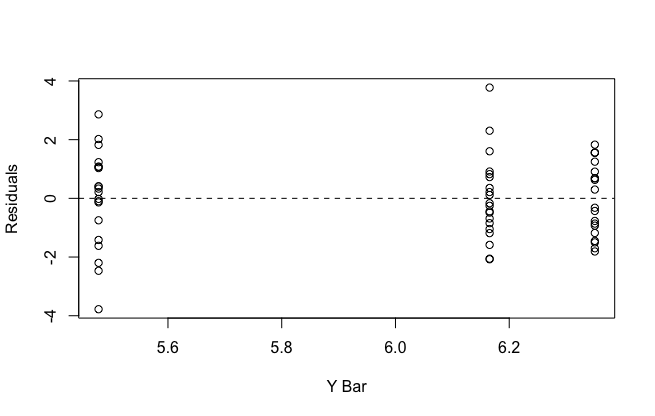
\includegraphics[scale=0.5]{lect-7-4-b.png}

\noindent In all these three levels, the residuals distribute randomly across the x-axis, therefore, the equivalent variance assumption is not violated. 

\subsection*{c}

\begin{figure}[!htb]
\minipage{0.32\textwidth}
  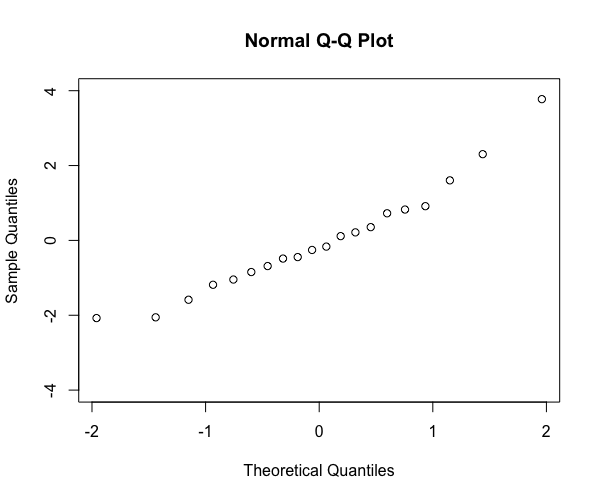
\includegraphics[width=\linewidth]{lect-7-4-c-1.png}
  \caption{1 hour}
\endminipage\hfill
\minipage{0.32\textwidth}
  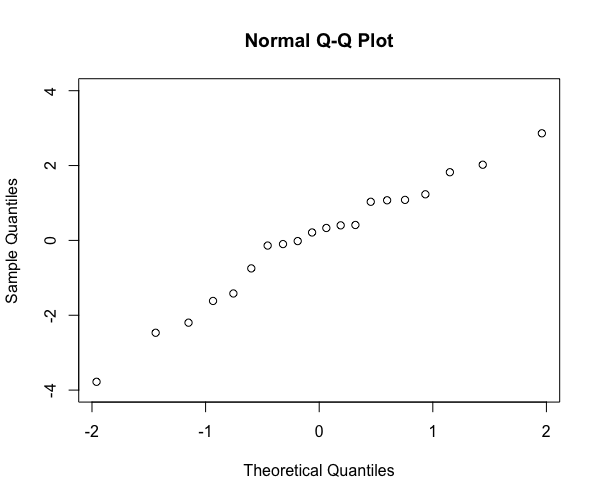
\includegraphics[width=\linewidth]{lect-7-4-c-2.png}
  \caption{2 hours}
\endminipage\hfill
\minipage{0.32\textwidth}%
  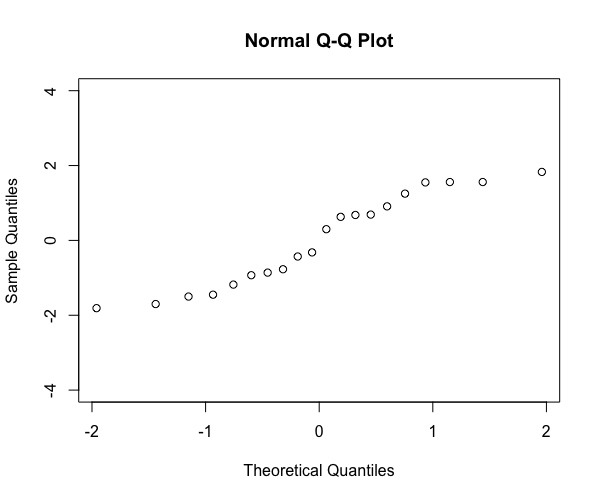
\includegraphics[width=\linewidth]{lect-7-4-c-3.png}
  \caption{4 hours}
\endminipage
\end{figure}
\noindent 

\begin{verbatim}
dt_1 <- data.frame(A, lm_1$residuals)
qqnorm(dt_1[dt_1$A==1,]$lm_1.residuals, ylim=c(-4, 4))
qqnorm(dt_1[dt_1$A==2,]$lm_1.residuals, ylim=c(-4, 4))
qqnorm(dt_1[dt_1$A==4,]$lm_1.residuals, ylim=c(-4, 4))
\end{verbatim}

\noindent We may perceive that the slope of third qqplot is slightly different from other two, but in general, their have similar slopes, therefore, equivalent variance assumption is not violated.

\subsection*{d}
\noindent Given the assumption that $Y_{ij} \sim N(\mu_i, \sigma_{\epsilon})$, by CLT, $\bar{Y_{i.}} \sim N(\mu_i, \frac{\sigma}{\sqrt{n}})$. \\
\noindent Since $\sigma_{\epsilon}^2$ is unknown, we use $MSE = \frac{\sum_i^a s_i^2}{a}$ as an estimator of $\sigma_{\epsilon}^2$. \\
\noindent Therefore, $\frac{\bar{Y_{i.}} - \mu_i}{\sigma / \sqrt{n}} \sim t_{N-a}$\\
\noindent CI for $\mu_i$ is $\bar{Y_{i.}} \pm t_{\alpha / 2, N-a} \cdot \sqrt{MSE / n}$
\begin{verbatim}
alpha <- 0.05
n <- 20
y1_mean <- mean(y_m[1,])
y_sds <- apply(y_m, 1, sd)
MSE <- sum(y_sds^2) / 3
cv_low <- y1_mean + sqrt(MSE / n) * qt(alpha/2, df=(60-3))
cv_high <- y1_mean - sqrt(MSE / n) * qt(alpha/2, df=(60-3))

> cv_high
[1] 6.814768
> cv_low
[1] 5.516232
\end{verbatim}
We are $95 \%$ confident $\mu_1$ is in the interval $[5.516232, 6.814768]$.

\subsection*{e}
\noindent Before applying t-test on $\mu_2 - \mu_3$, we need to check if their population variance is the same. A two variance F-test is applied here. 
\begin{verbatim}
y2_sd <- sd(y_m[2,])
y3_sd <- sd(y_m[3,])
F_obs <- y2_sd^2 / y3_sd^2
p_val <- pf(1 - (F_obs-1), df1=n-1, df2=n-1) +
  (1 - pf(F_obs, df1=n-1, df2=n-1))
  
> p_val
[1] 0.1091745
\end{verbatim}
\noindent The p-value of F-statistic is 0.109, which is not a strong evidence against equivalent variance assumption. Therefore, t-test can be done on these two population means. \\

\noindent CI for $\mu_i - \mu_j$ is $(\bar{Y_{i.}} - \bar{Y_{j.}}) \pm t_{\alpha / 2, N-a} \cdot \sqrt{2MSE / n}$
\begin{verbatim}
y2_mean <- mean(y_m[2,])
y3_mean <- mean(y_m[3,])
cv_low <- y2_mean - y3_mean + sqrt(2 * MSE / n) * qt(alpha/2, df=(60-3))
cv_high <- y2_mean - y3_mean - sqrt(2 * MSE / n) * qt(alpha/2, df=(60-3))

> cv_low
[1] -1.790704
> cv_high
[1] 0.04570407
\end{verbatim}
We are $95 \%$ confident that $\mu_2 - \mu_3$ is in the interval $[-1.790704, 0.04570407]$.

\subsection*{f}
$\Gamma = \mu_1 - \frac{1}{2} \mu_2 - \frac{1}{2} \mu_3$, $\vec{c} = (1, -\frac{1}{2}, -\frac{1}{2})$ \\

\noindent $H_0: \Gamma = 0$, $H_1: \Gamma \neq 0$, assume $\sigma_1 = \sigma_2 = \sigma_3$\\

\noindent We use $\hat{\Gamma} = \sum_i^a c_i \bar{Y_i}$ as an unbiased estimator for $\Gamma$, $MSE = \frac{1}{a} \sum_i^a s_i^2$ as an estimator for $\sigma_{\epsilon}^2$. \\

\noindent $t = \frac{\hat{\Gamma} - \Gamma_0}{\sqrt{Var(\hat{\Gamma})}} = \frac{\hat{\Gamma} - \Gamma_0}{\sqrt{MSE \cdot \sum_i^a c_i^2 / n}} \sim t_{N-a}$ \\

\noindent We will reject $H_0$ in favor of $\Gamma \neq 0$ if t-statistic $t > t_{1-\frac{\alpha}{2}, N-a}$ or $t < t_{\frac{\alpha}{2}, N-a}$
\begin{verbatim}
c <- c(1, -1/2, -1/2)
gamma_est <- sum(y_bars * c)
MSE <- sum(y_sds^2) / 3
t <- gamma_est / (sqrt(MSE * sum(c^2) / n))
low_cv <- qt(alpha/2, df=n*3 - 3)
up_cv <- qt(1-alpha/2, df=n*3 - 3)

> t
[1] 0.632705
> low_cv
[1] -2.002465
> up_cv
[1] 2.002465
\end{verbatim}
\noindent The rejection regions are $t < -2.002465$ or $t > 2.002465$, the t-statistic from observed values (0.632705) does not fall in any of these regions, therefore, under significant level of $0.05$, the contrast test fail to provide strong evidence against $H_0$. 

\subsection*{g}
\begin{align*}
& P(t_{\frac{1}{2} \alpha, N-a} < t < t_{ 1 - \frac{1}{2} \alpha, N-a}) = 1 - \alpha \\
& P(t_{\frac{1}{2} \alpha, N-a} < \frac{\hat{\Gamma} - \Gamma_0}{\sqrt{MSE \cdot \sum_i^a c_i^2 / n}} < t_{ 1 - \frac{1}{2} \alpha, N-a}) = 1 - \alpha \\
& P( \hat{\Gamma} + t_{\frac{1}{2} \alpha, N-a} \sqrt{MSE \cdot \sum_i^a c_i^2 / n} < \Gamma <  \hat{\Gamma} - t_{\frac{1}{2} \alpha, N-a} \sqrt{MSE \cdot \sum_i^a c_i^2 / n} ) = 1 - \alpha
\end{align*}
\begin{verbatim}
ci_low <- gamma_est + (sqrt(MSE * sum(c^2) / n)) * qt(alpha/2, df=n*3 - 3)
ci_up <- gamma_est - (sqrt(MSE * sum(c^2) / n)) * qt(alpha/2, df=n*3 - 3)

> ci_low
[1] -0.5439381
> ci_up
[1] 1.046438
\end{verbatim}
\noindent We are $95\%$ confident that $\Gamma$ is in the interval $[-0.5439381,1.046438 ]$ as computed from observed data. Since this CI include the null hypothesis value $\Gamma = 0$, this constant test fail to show strong evidence against $H_0$. 

\subsection*{Lect 8-1}
\subsection*{a}
$H_0: \mu_1 = \mu_2 = \mu_3$, $H_1:$ there are at least two means are different. 
\begin{verbatim}
a <- 3
n <- 5
ct_m <- matrix(nrow=a, ncol=n)
ct_m[1,] <- c(9 ,12, 10, 8, 15)
ct_m[2,] <- c(20, 21, 23, 17, 30)
ct_m[3,] <- c(6, 5, 8, 16, 7)
y_means <- apply(ct_m, 1, mean)
grand_mean <- mean(ct_m)
y_sds <- apply(ct_m, 1, sd)
SStr <- n * sum((y_means - grand_mean)^2)
SSe <- (n-1) * sum(y_sds^2)
F_obs <- (SStr / (a-1)) / (SSe / (n*a - a))
p_val <- pf(F_obs, df1=a-1, df2=a*n - a, lower.tail = F)

> SStr
[1] 543.6
> SSe
[1] 202.8
> F_obs
[1] 16.08284
> p_val
[1] 0.0004023258
\end{verbatim}
\noindent Observed f-statistic is $16.08284$, which has a p-value of $0.0004023258$, much less than $0.001$. This one way ANOVA F-test provides significant evidence against $H_0$ in favor of the alternative that there exist at least two means are different. 

\subsection*{b}
\begin{verbatim}
A <- as.factor(rep(c(1,2,3), each=n))
ct <- as.vector(t(ct_m))
lm_2 <- lm(ct~A)
aov(ct~A)
summary.aov(lm_2)
\end{verbatim}
\noindent By $lm()$, SStreat = 543.6, SSe = 202.8, F-statistic = 16.08, and p-value = 0.000402. Conclusion is same as above. 

\subsection*{c}
\noindent Apply a F-test on $H_0: \sigma_1 = \sigma_3$, $H_1: \sigma_1 \neq \sigma_3$
\begin{verbatim}
y1_sd <- sd(ct_m[1,])
y3_sd <- sd(ct_m[3,])
F_obs <- y1_sd^2 / y3_sd^2
p_val <- (1 - pf(1 + (1 - F_obs), df1=n-1, df2=n-1)) +
  pf(F_obs, df1=n-1, df2=n-1)
  
> p_val
[1] 0.5273811
\end{verbatim}
\noindent The p-value is 0.5273811, which is much greater than 0.05, indicating that sample data fail to provide strong evidence against equivalent variances assumption. A two-sample t-test can be applied here. \\

\noindent CI for $\mu_1 - \mu_3$ is $(\bar{Y_{1.}} - \bar{Y_{3.}}) \pm t_{\alpha / 2, N-a} \cdot \sqrt{2MSE / n}$
\begin{verbatim}
MSE <- sum(y_sds^2) / a
y1_bar <- mean(ct_m[1,])
y3_bar <- mean(ct_m[3,])
ci_low <- (y1_bar - y3_bar) + qt(alpha/2, df=a*(n-1)) * sqrt(2 * MSE / n)
ci_up <- (y1_bar - y3_bar) - qt(alpha/2, df=a*(n-1)) * sqrt(2 * MSE / n)

> ci_low
[1] -3.264913
> ci_up
[1] 8.064913
\end{verbatim}

\noindent We are $95 \%$ confident that $\mu_1 - \mu_3$ is in the interval [-3.264913, 8.064913]. Since this interval covers 0, the observed data fail to provide evidence against $H_0$. 

\subsection*{d}
\noindent $H_0: \mu_1 - \mu_3 = 0$, $H_1: \mu_1 - \mu_3 \neq 0$ \\

\noindent under the null hypothesis, $t_obs = \frac{\bar{Y_1.} - \bar{Y_3.}}{\sqrt{2 \cdot  MSE / n}} \sim t_{N-a}$

\begin{verbatim}
t_obs <- (y1_bar - y3_bar) / sqrt(2 * MSE / n)
p_val <- 2 * (1 - pt(t_obs, df=n*a - a))

> p_val
[1] 0.374155
\end{verbatim}
\noindent Under the null hypothesis, p-value of observed t is 0.374155, greater than 0.05. Therefore, the sample fail to provide strong evidence against equivalent means. 

\subsection*{e}
\noindent In part b, $H_0: \mu_1 - \mu_3$, $\vec{c} = (1, 0, -1)$, another orthogonal vector is $\vec{d} = (1, -2, 1)$
\begin{verbatim}
u <- c(-1, 0, 1, 0)
v <- c(-1, 2, -1, 0)
w <- c(-1, -1, -1, 3)
u_ssc <- (sum(u * y_bars))^2 / (sum(u^2) / n)
v_ssc <- (sum(v * y_bars))^2 / (sum(v^2) / n)
w_ssc <- (sum(w * y_bars))^2 / (sum(w^2) / n)
sum(c(u_ssc, v_ssc, w_ssc))

> c(c_ssc, d_ssc)
[1] 14.4 529.2
> sum(c(c_ssc + d_ssc))
[1] 543.6
\end{verbatim}
\noindent Sum of contrast sum of squares is equal to $SS_{tr}$.

\subsection*{f}
\begin{verbatim}
> c(c_ssc, d_ssc)
[1] 14.4 529.2
\end{verbatim}
\noindent In ANOVA F-test, larger $SS_{tr}$ will lead to more statistical significance (smaller p-value). Since the second contrast vector contributes more to the $SS_{tr}$, we can say the second contrast vector is contributing more to significance. 

\subsection*{g}
\noindent $H_0: \Gamma = 0$, $H_1: \Gamma \neq 0$
\begin{align*}
t_obs &= \frac{\hat{\Gamma} - \Gamma_0}{\sqrt{MSE \cdot |\vec{c}| / n  }} \sim t_{N-a} \\
\hat{\Gamma} &= \sum_i^a c_i \cdot \bar{Y_{i.}}, \Gamma_0 = 0
\end{align*}
\noindent For vector $\vec{c} = (1, 0, -1)$
\begin{verbatim}
c <- c(1, 0, -1)
MSE <- sum(y_sds^2) / a
c_gamma <- sum(c * y_means)
t_obs <- c_gamma / sqrt(MSE * sum(c^2) / n)
p_val <- 2 * (1 - pt(t_obs, df=n * (a-1)))

> p_val
[1] 0.3777015
\end{verbatim}
\noindent $\hat{\Gamma} = 2.4$, with p-value of 0.378, which is greater than 0.05. This contrast test fail to provide significant evidence against $H_0: \Gamma = 0$. \\

\noindent For vector $\vec{d} = (1, -2, 1)$
\begin{verbatim}
d <- c(1, -2, 1)
d_gamma <- sum(d * y_means)
t_obs <- d_gamma / sqrt(MSE * sum(d^2) / n)
p_val <- 2 * pt(t_obs, df=n * (a-1))

> p_val
[1] 0.0002290025
\end{verbatim}
\noindent By this contrast, $\hat{\Gamma} = -25.2$, with p-value of 0.00023, which is much less than 0.05. This contrast test provides significant evidence against $H_0$, in favor of $\Gamma \neq 0$.

\subsection*{Lect 8-2}
\noindent $c_i$'s, $\mu_i$'s are constant, assume $\epsilon$ iid, $\epsilon \sim N(0, 1)$, $E(\epsilon_{ij}) = E(\epsilon) = 0$, $Var(\epsilon_{ij}) = Var(\epsilon) = \sigma_{\epsilon}^2$
\begin{align*}
E(SS_c) &= E( \frac{(\sum_i^a c_i \bar{Y_{i.}})^2}{|\vec{c}|^2 / n} ) \\
&= \frac{1}{|\vec{c}|^2 / n} E((\sum_i^a c_i \bar{Y_{i.}})^2 ) \\
&= \frac{1}{|\vec{c}|^2 / n} (Var(\sum_i^a c_i \bar{Y_{i.}}) + E(\sum_i^a c_i \bar{Y_{i.}})^2) 
\end{align*}
\begin{align*}
Var(\sum_i^a c_i \bar{Y_{i.}}) &= \sum_i^a c_i^2 \cdot  Var( \bar{Y_{i.}} ) \\
&= \sum_i^a c_i^2 \cdot Var(\frac{1}{n} \sum_j^n \mu_i + \epsilon_{ij}) \\
&= \sum_i^a c_i^2 \cdot Var(\frac{1}{n} \sum_j^n  \epsilon_{ij}) \\
&= \frac{1}{n^2} \sum_i^a c_i^2 \cdot \sum_j^n Var(\epsilon_{ij}) \\
&= \frac{1}{n^2} \sum_i^a c_i^2 \cdot \sigma_{\epsilon}^2 \sum_j^n 1 \\
&= \frac{1}{n} | \vec{c} |^2  \cdot \sigma_{\epsilon}^2
\end{align*}
\begin{align*}
E(\sum_i^a c_i \bar{Y_{i.}} ) &= \sum_i^a c_i E(\bar{Y_{i.}}) \\
&= \sum_i^a c_i E(\frac{1}{n} \sum_j^n \mu_i + \epsilon_{ij}) \\
&= \sum_i^a c_i (\mu_i + \frac{1}{n} \sum_j^n E(\epsilon_ij)) \\
&= \sum_i^a c_i (\mu_i ) = \Gamma
\end{align*}
\begin{align*}
E(SS_c) &= \frac{1}{|\vec{c}|^2 / n} (Var(\sum_i^a c_i \bar{Y_{i.}}) + E(\sum_i^a c_i \bar{Y_{i.}})^2) \\
&= \frac{1}{|\vec{c}|^2 / n} \cdot \frac{1}{n} | \vec{c} |^2  \cdot \sigma_{\epsilon}^2 + \frac{1}{|\vec{c}|^2 / n} \cdot \Gamma^2 \\
&= \sigma_{\epsilon}^2 + \frac{\Gamma^2}{|\vec{c}|^2 / n}
\end{align*}

\subsection*{Lect 8-3}
\subsection*{a}
\begin{verbatim}
a = 4
n = 4
y_m <- matrix(nrow=a, ncol=n)
y_m[1,] = c(143, 141, 150, 146)
y_m[2,] = c(152, 149, 137, 143)
y_m[3,] = c(134, 136, 132, 127)
y_m[4,] = c(129, 127, 132, 129)
c <- c(1, 1, -1, -1)
d <- c(1, -1, 0, 0)
e <- c(0, 0, 1, -1)
y_bars <- apply(y_m, 1, mean)
c_ssc <- (sum(c * y_bars))^2 / (sum(c^2) / n)
d_ssc <- (sum(d * y_bars))^2 / (sum(d^2) / n)
e_ssc <- (sum(e * y_bars))^2 / (sum(e^2) / n)

> c(c_ssc, d_ssc, e_ssc)
[1] 826.5625   0.1250  18.0000
> sum(c(c_ssc, d_ssc, e_ssc))
[1] 844.6875
\end{verbatim}
\noindent Sum of three contrast sum of squares is equal to $SS_{tr}$

\subsection*{b}
\noindent choose $\vec{f} = (1, -1, 1, -1)$, $\vec{g} = (0, 1, 0, -1) $, $\vec{h} = (1, 0, -1, 0)$
\begin{verbatim}
f <- c(1, -1, 1, -1)
g <- c(0, 1, 0, -1) 
h <- c(1, 0, -1, 0)
f_ssc <- (sum(f * y_bars))^2 / (sum(f^2) / n)
g_ssc <- (sum(g * y_bars))^2 / (sum(g^2) / n)
h_ssc <- (sum(h * y_bars))^2 / (sum(h^2) / n)

> c(f_ssc, g_ssc, h_ssc)
[1] 7.5625 512.0000 325.1250
> sum(c(c_ssc, g_ssc, h_ssc))
[1] 844.6875
\end{verbatim}
\noindent Sum of three contrast sum of squares is equal to $SS_{tr}$

\subsection*{c}
\noindent choose $\vec{u} = (-1, 0, 1, 0)$, $\vec{v} = c(-1, 2, -1, 0)$, $\vec{w} = c(-1, -1, -1, 3)$
\begin{verbatim}
u <- c(-1, 0, 1, 0)
v <- c(-1, 2, -1, 0)
w <- c(-1, -1, -1, 3)
u_ssc <- (sum(u * y_bars))^2 / (sum(u^2) / n)
v_ssc <- (sum(v * y_bars))^2 / (sum(v^2) / n)
w_ssc <- (sum(w * y_bars))^2 / (sum(w^2) / n)

> c(u_ssc, v_ssc, w_ssc)
[1] 325.1250 117.0417 402.5208
> sum(c(u_ssc, v_ssc, w_ssc))
[1] 844.6875
\end{verbatim}
\noindent Sum of three contrast sum of squares is equal to $SS_{tr}$

\end{document}